\section{Методы анализа сортировок за квадратное время}
\epigraph{Если мы скажем, что проходим на лекции бабл сорт, то нас засмеют, поэтому назовем нашу лекцию так.}
{Г.О. Евстропов}

В процессе анализа алгоритма мы будем доказывать \textit{корректность} алгоритма и анализировать \textit{время его работы}. \par

Существуют хотя бы три метода доказательства корректности алгоритма (нам их должно хватить):
\begin{enumerate}
    \item по индукции;
    \item от противного;
    \item поиск инварианта.
\end{enumerate}

\begin{definition}
    «Задача о сортировке». Есть $n$ произвольных элементов $a_1, \ldots, a_n$. Хочется их упорядочить так, чтобы $a_{\pi(1)} \leq a_{\pi(2)} \leq \ldots \leq a_{\pi(n)}$.
\end{definition}

\textbox{
    \medskip
    \textbf{\large Лирическое отступление: RAM-модель} \par
    В нашей RAM-подели будет:
    \begin{itemize}
        \item 
            \begin{tikzpicture}
                \draw (0, 0) rectangle (0.3, 0.3);
            \end{tikzpicture}
            -- процессор. За единицу времени он умеет выполнять одно действие с целочисленными данными, а также запрос к одной ячейке пямяти.

        \item 
            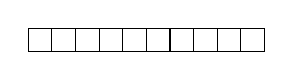
\begin{tikzpicture}
                \draw [step=0.3cm] (0, 0) grid (3, 0.3);
            \end{tikzpicture}
            -- память. Её всегда ассимпотически достаточно для любых действий (но не слишком много). Например, при $P(n)$ действий памяти будет примерно $c \cdot P(n)$. Кроме того, любая работа с куском памяти выполняется не быстрее, чем за длину этого куса.
    \end{itemize}

    Что мы умеем хранить и делать в RAM-модели:
    \begin{itemize}
        \item целые числа;
        \item вещественные числа;
        \item $\pm, \ *, /, \%$ за $O(1)$;
        \item все битовые операции выполняются за $O(1)$;
        \item всякие $\sqrt{x}, \sin{x}, \cos{x}, \ldots$ мы тоже умеем вычислять за $O(1)$ (если противное не оговорено заранее).
    \end{itemize}
}

\newpage
\subsection{Сортировка пузырьком (bubble sort)}

    \begin{algorithm}
        \caption{Bubble sort}
        \begin{algorithmic}
            \While{\Call{not\_sorted}{}}
                \For{$i: 1 \to n - 1$}
                    \If{$a_i > a_{i+1}$}
                        \Call{swap}{$a_i, a_{i+1}$}
                    \EndIf
                \EndFor
            \EndWhile
        \end{algorithmic}
    \end{algorithm}

    Теперь нужно доказать корректность алгоритма.
    \begin{proof_cor}
        На каждом шаге количество инверсий уменьшается хотя бы на $1$, а значит за конечное число итераций алгоритм закончится.
    \end{proof_cor}

    Оценим количество операций. Оно, очевидно, не превосходит количество инверсий, а их не более, чем $\frac{n(n+1)}{2}$. \par

\subsection{Сортировка выбором}
    \begin{algorithm}
        \caption{Selection sort}
        \begin{algorithmic}
            \For{$i: n \to 1$}
                \Let{p}{\Call{select\_max}}{$(1, i)$}
                \State \Call{swap}{$a_p, a_i$}
            \EndFor
        \end{algorithmic}
    \end{algorithm}

    \begin{algorithm}
        \caption{Selection sort (recursive)}
        \begin{algorithmic}
            \Function{rec}{$a, n$}
                \If{$n = 1$} \Return \EndIf
                \Let{p}{\Call{select\_max}}{$1, i$}
                \State \Call{swap}{$a_p, a_i$}
                \State \Call{rec}{$a, n - 1$}
            \EndFunction
        \end{algorithmic}
    \end{algorithm}    

    \begin{proof_cor}
        Докажем корректность индукцией по $n$.
        
        \begin{enumerate}
            \item База. $n = 1$. Один элемент уже отсортирован.
            \item Допустим, для какого-то $n$ алогоритм работает корректно, то есть сортировка работает для всех массивов длинны $n$. Рассмотрим массив из $n + 1$ элемента. Тогда на первой итерации алгоритма на место $a_{n+1}$ встанет максимальный элемент (то есть он встанет на своё место). Тогда после первой итерации в остальных $n$ элементах будут элементы меньше, чем $a_{n+1}$, а для них алогоритм работает корректно.
        \end{enumerate}
    \end{proof_cor}

    Теперь о времени работы. Докажем, что $t(n) \leq c_2 \cdot n^2$.

    \begin{proof_cor}
        Действительно, выразим величину $t(n)$ рекурсивно через прыдудещий шаг. На $n$-том шаге алгоритм ищет максимальный элемент (за $c_1 \cdot n$ времени). Тогда
        \[
            t(n) \leq c_1n + t(n-1).
        \]
        Воспользуемся индукцией по $n$. База очевидна, та что напишем переход:
        \[
            t(n) \leq c_1n + c_2(n-1)^2 = c_1n + c_2n^2 - 2nc_2 + c_2.
        \]
        Возьмем $c_2 = c_1$ (нам же нужно выбрать $c_2$ такой, что...).
        \note{Тут я не уверен.}
        Тогда
        \[
            t(n) \leq c_1n + c_1n^2 - 2nc_1 + c_1 = c_1n^2 + c_1 - c_1n \leq c_1n^2 = c_2n^2.
        \]
    \end{proof_cor}

\subsection{Сортировка вставками}

    \textit{Инвариант.} На $i$-том шаге алгоритма префикс до $i-1$-го элемента отсортирован.

    \begin{algorithm}
        \caption{Insertion sort}
        \begin{algorithmic}
            \For{$i:1 \to n$}
                \Call{insert}{$a, i, a_i$}
            \EndFor
        \end{algorithmic}
    \end{algorithm}

    \begin{proof_cor}
        Очевидно, что на $n + 1$ шаге весь префикс будет отсортирован, а функция $insert$ вставит элемент $a_{n+1}$ на своё порядковое место внутри этого префикса.
    \end{proof_cor}

    \begin{proof_time}
        Всего выполняется $n$ внешних итераций. Функция $insert$ в худшем случае (при вставке элемента в самое начало) работает за $i$ итераций, где $i$ -- длина префикса. Таким образом получается $\frac{n(n+1)}{2}$ итераций, а значит $t(n) = O(n^2)$. 
    \end{proof_time}

\subsection{Типы сортировок}
